\refstepcounter{chapter}
\addcontentsline{toc}{chapter}{Before Starting the Machine}
\section{Important Notes}

\subsection{Factory Number}
\begin{itemize}
    \item The information in this operator's manual applies \uline{\textbf{only}} to the machine whose factory number is stamped on the machine's nameplate.
    \item For all inquiries and spare part orders, the factory number of the machine must be specified.
    \item If inquiries pertain to a specific page of the operator's manual, the page number must also be provided.
\end{itemize}

\subsection{Before Starting the Machine}
\begin{itemize}
    \item Carefully read the operator's manual.
    \item Set up the machine (see Page 1.03-1).
    \item Ensure that the machine has reached room temperature.
    \item Remove rust protection (see Page 1.08-1).
    \item Tighten all terminal screws on the terminal strips, contactors, relays, and fuses in the control cabinet; they may have loosened due to vibrations during transport.
    \item Connect the machine to the electrical network (see Page 1.10-1).
    \item Check oil levels (see Page 7.02-1 and 7.03-1).
    \item Fill the machine with coolant (see Page 3.22-1).
\end{itemize}

\subsection{Interlocks of the Machine}
\begin{itemize}
    \item After switching off the main switch -Q1- in the control cabinet and after every power failure, the machine must be restarted.\footnote{"Start the machine", see separate CNC 432 operating instructions.}
    \item The red mushroom button of the EMERGENCY STOP switch must not be pressed during this process.
    \item After each EMERGENCY STOP, the corresponding mushroom button must be \\released by turning it clockwise, and the machine must be restarted.\textsuperscript{\thefootnote}
\end{itemize}

\section{Transport of the Machine}

The dimensions and weights of the machine with the fixed table and coolant container are as follows:

\begin{table}[h]
\centering
\begin{tabular}{lll}
\textbf{Packaging Type} & \makecell{\textbf{Dimensions}\\\textbf{(L x W x H) [m]}} & \textbf{Weight [kg]} \\ \hline
EURO Packaging (Pallet/Carton) & $1.9 \times 1.8 \times 2$ & 1450 \\
Box (USSR) & $1.9 \times 1.9 \times 2.05$ & 1590 \\
Box (Seaworthy) & $2.35 \times 1.9 \times 2.05$ & 1693 \\
Container Loading (Machine on Pallet) & $1.8 \times 1.8 \times 1.98$ & 1362 \\
\end{tabular}
\end{table}

\begin{figure}[h]
    \centering
    \begin{minipage}[b]{0.35\textwidth} % Align to the bottom with [b]
        \centering
        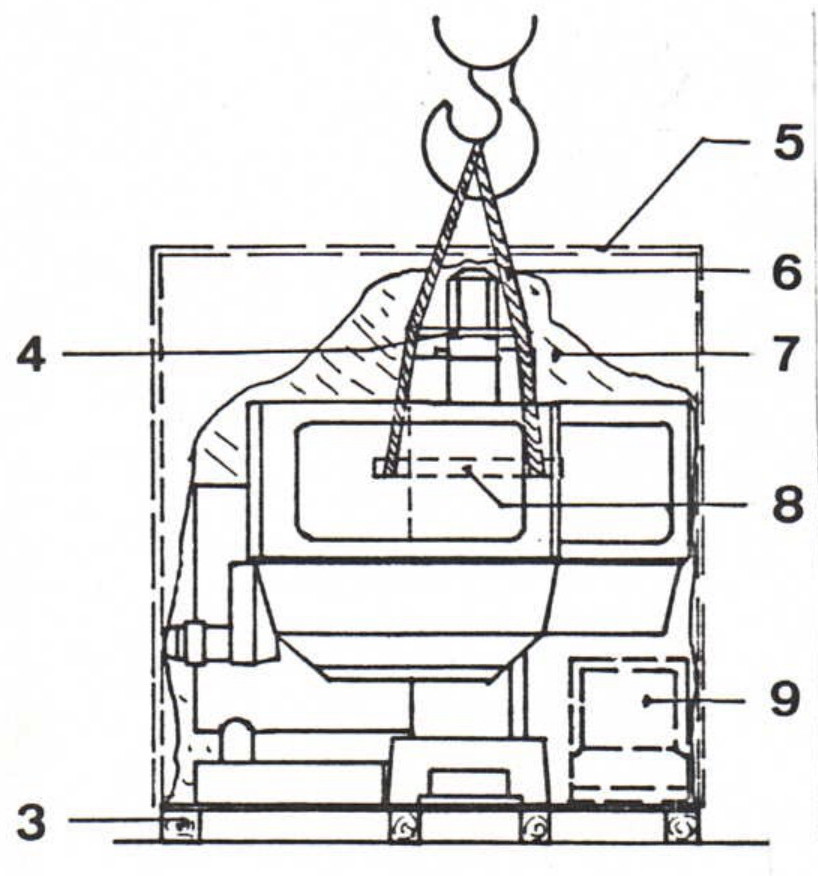
\includegraphics[width=\textwidth]{machine_packaging_transport.jpg} % Replace with actual image file
        \caption{}
        \label{fig:packaging}
    \end{minipage}
    \hfill
    \begin{minipage}[b]{0.55\textwidth} % Align to the bottom with [b]
        \centering
        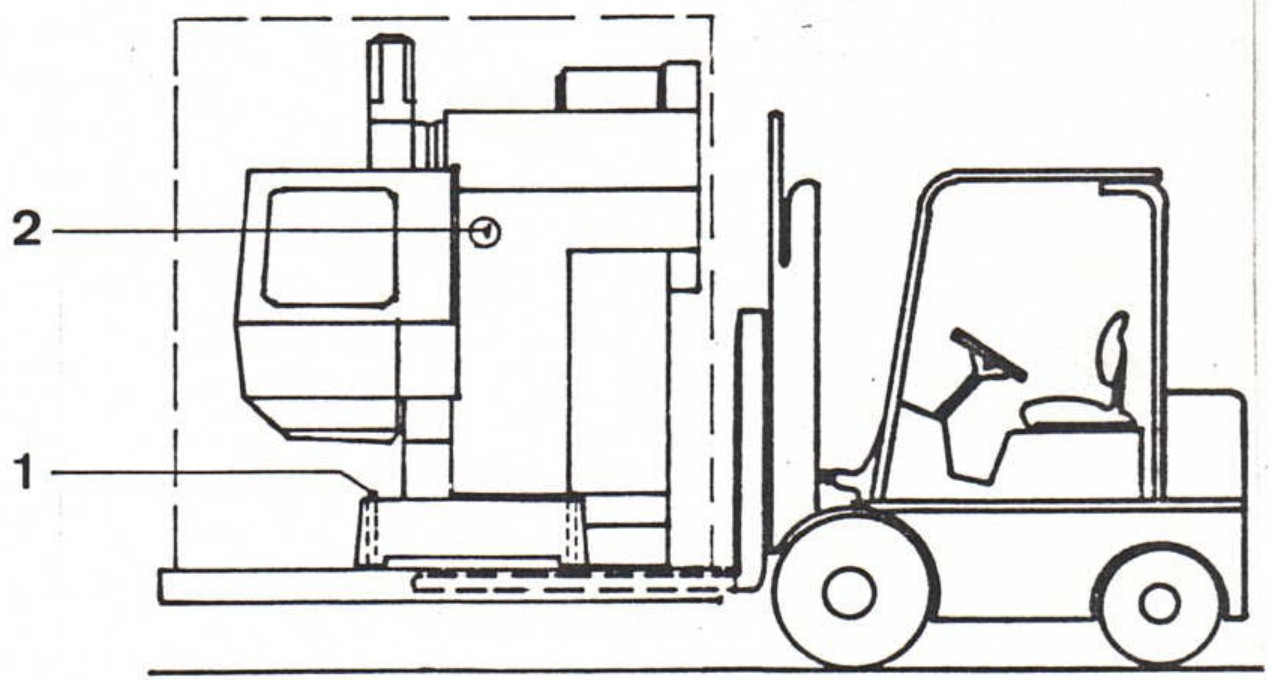
\includegraphics[width=\textwidth]{machine_unloading_forklift.jpg} % Replace with actual image file
        \caption{}
        \label{fig:unloading}
    \end{minipage}
    \end{figure}

\begin{itemize}
    \item Unload the packaged machine from the transport device using a forklift, hoist, or similar equipment.
    \item Remove the packaging (\textbf{5}) and cut and remove the protective foil (\textbf{7}) from the base of the box. Take off the sealing covers (\textbf{2}) on both sides.
    \item Check the machine and accessories for any transport damage.
\end{itemize}

\notebox{NOTE}{Damages or other defects, such as incompleteness, must be reported immediately in writing to the shipping company or railway, the insurance company, and the company MAHO.} 

\begin{itemize}
    \item Insert the transport rod (\textbf{8}) (maximum 50 mm diameter, 1000 mm length) into the opening in the stand.
    \item Attach the endless sling (\textbf{6}), with a minimum load capacity of 3000 kg and a total length of approximately 6 m, to the crane hook and the transport rod.
\end{itemize}

\notebox{CAUTION}{Place the detached control panel (\textbf{9}) on the work table and secure it against slipping!}

\subsection{\MakeUppercase{\textbf{\uline{Transport of the Machine}}}}

\begin{itemize}
    \item Perform a hanging test, i.e., align the machine by moving the transport rod (\textbf{8}) in the stand so that it hangs horizontally. Using a spacer (\textbf{4}) prevents the rope from rubbing against the machine.
    
    \item Lower the machine, unscrew the fastening nuts (\textbf{1}), and remove the pallet or box bottom (\textbf{3}) after lifting the machine again.
\end{itemize}

\noindent\textbf{When using a forklift:} Place the machine on wooden boards laid on the forks of the forklift (Fig. \ref{fig:unloading}) or hang it on the forks using a rope (Fig. \ref{fig:machine_placement_forklift}).
    
\vspace{1em} % Use this for spacing instead of \\

\noindent In unfavorable space conditions, use the "Transport Mule" (Fig. \ref{fig:machine_placement_mule}).

\begin{itemize}
    \item Transport the machine to the prepared location according to Page 1.03-1 and carefully place it on the damping plates provided.
\end{itemize}

\begin{figure}[h]
\centering
\begin{minipage}[t]{0.45\textwidth}
    \centering
    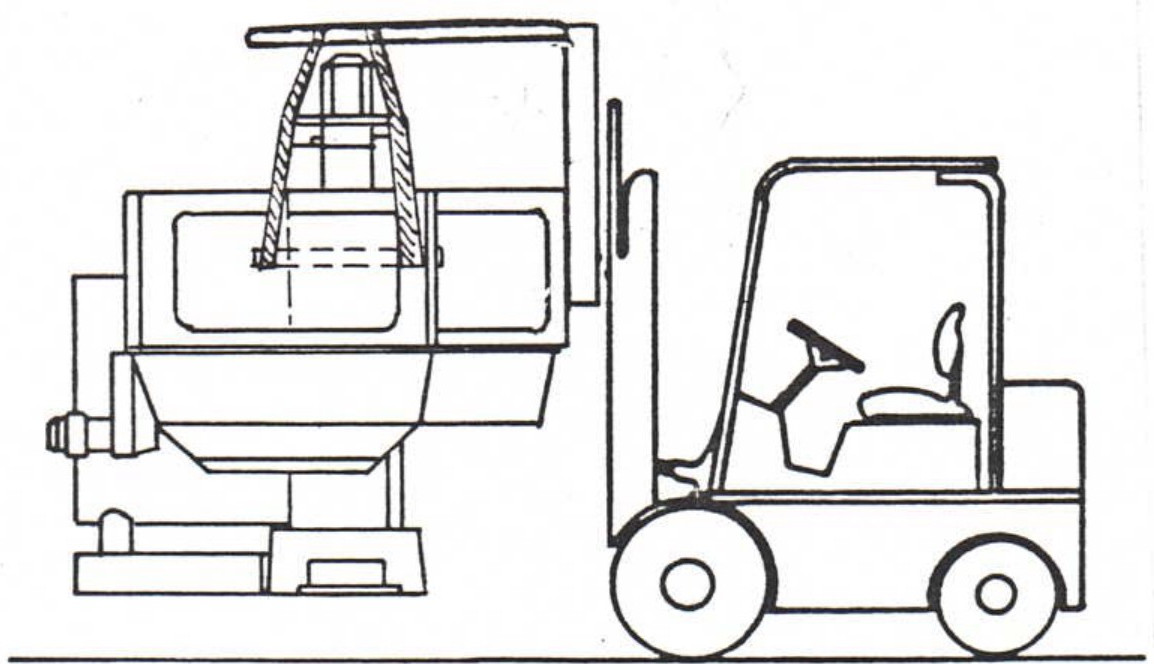
\includegraphics[width=\textwidth]{machine_placement_forklift.jpg} % Replace with actual image file
    \caption{}
    \label{fig:machine_placement_forklift}
\end{minipage}
\hfill
\begin{minipage}[t]{0.45\textwidth}
    \centering
    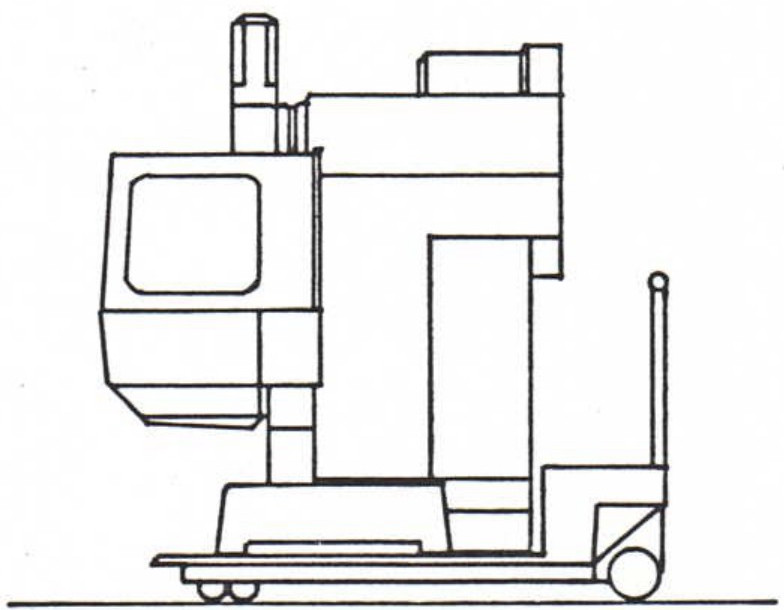
\includegraphics[width=\textwidth]{machine_placement_mule.jpg} % Replace with actual image file
    \caption{}
    \label{fig:machine_placement_mule}
\end{minipage}
\end{figure}

\vspace{1em}

\infoBullet{Setup plan and workspace layout}{1.04-1}
